\section{Serial Communication \refskript{9.1}}

\begin{itemize}
	\itemsep-.5em 
	\item \textbf{Parallel} n bits are transferred simultaneously in parallel
	\item \textbf{Serial} n bits are transferred serially, i.e., one after the other \\ Minimal duration of transfer: $n \cdot t_{Bit}$
\end{itemize}

\subsection{Types of Serial Channels \refskript{9.2}}
\begin{itemize}
	\itemsep-.5em 
	\item Simplex
	\item Half duplex
	\item Full duplex
\end{itemize}

\subsubsection{Serial Channel Topologies}
\begin{center}
	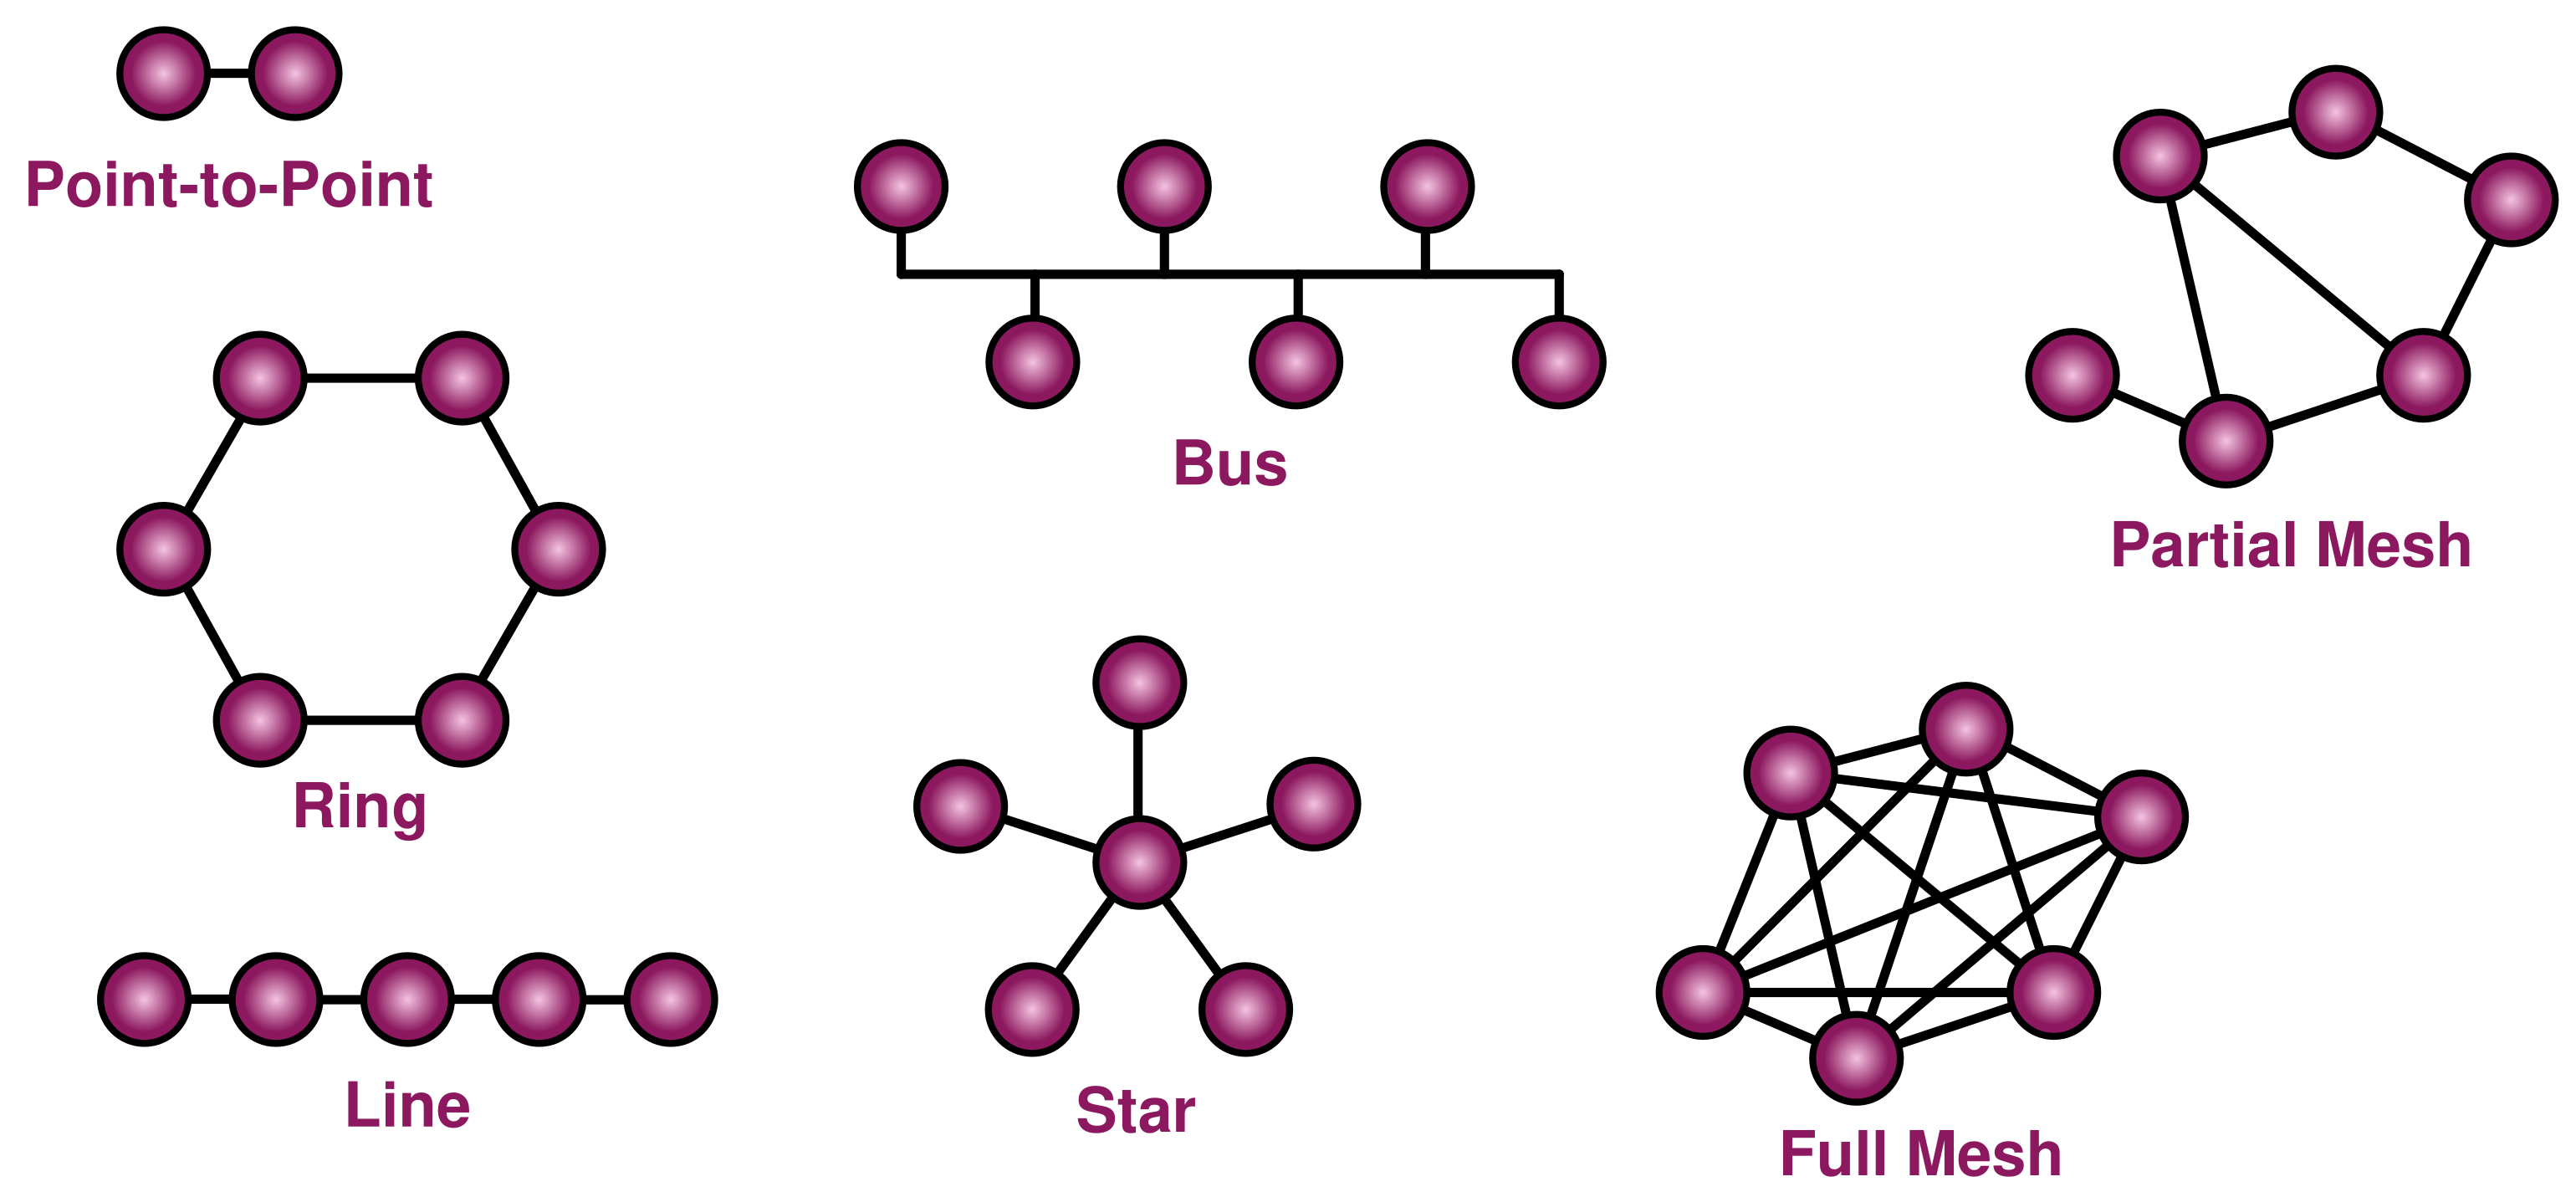
\includegraphics[width=.9\columnwidth]{"Images/Serial_Channel_Topologies.png"}
\end{center}


\subsection{Asynchronous Serial Communication \refskript{9.3}}
Asynchronous Packet Format \refskript{9.3.2}\\
\begin{itemize}
	\itemsep-.5em 
	\item \textbf{Header} 1 Start bit
	\item \textbf{Body} 5 to 8 bits character (LSB first)
	\item optional 1 parity bit
	\item \textbf{Footer} 1/1.5/2 Stop bits
\end{itemize}
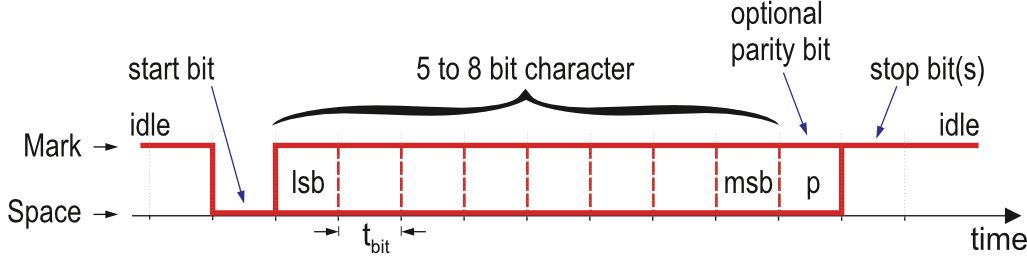
\includegraphics[width=\columnwidth]{"Images/async_package_format.png"}

Both Devices (Sender and Receiver) have there own clock generators that must be synchronized regularly.

Bit-Sampling at Receiver-Side: Too Slow
\begin{center}
	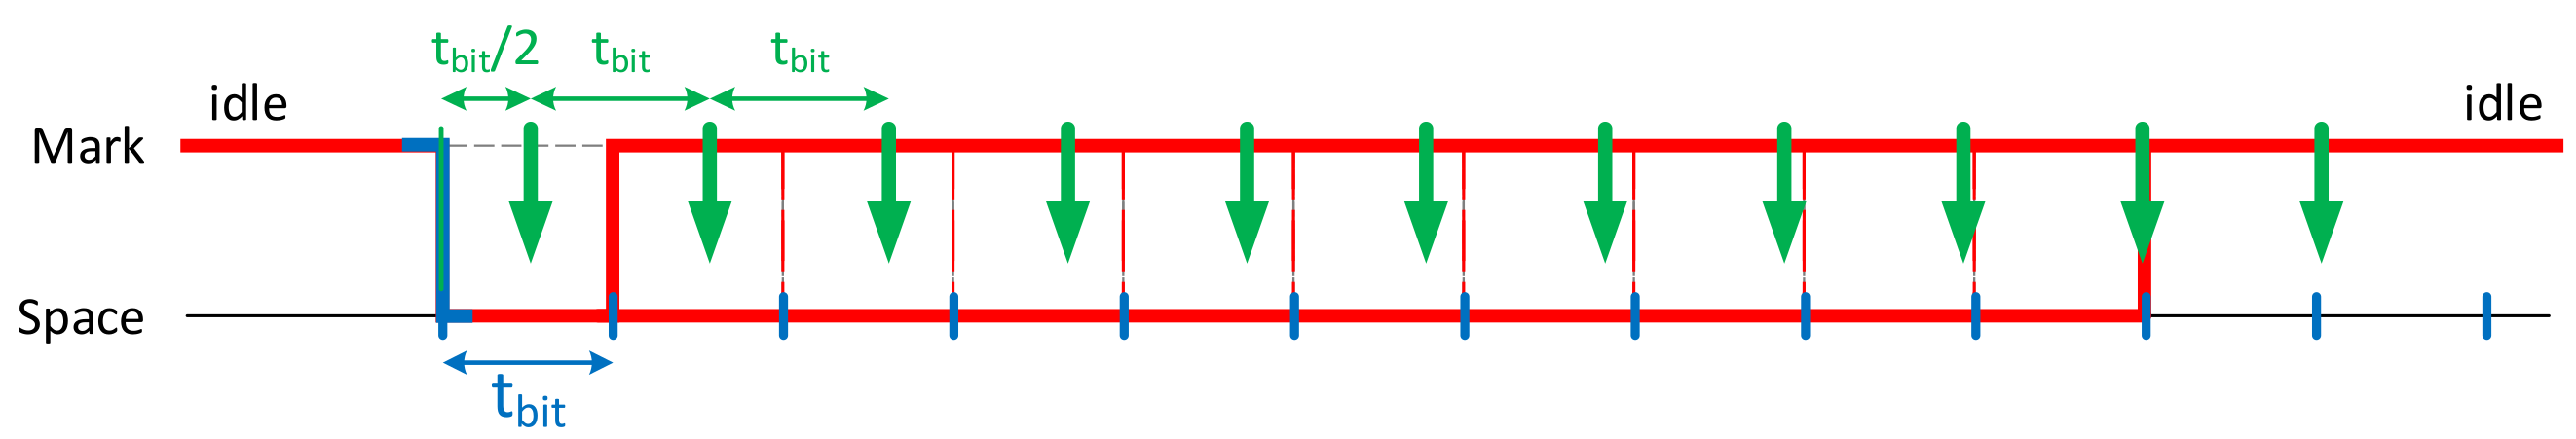
\includegraphics[width=.9\columnwidth]{"Images/bit_smapling.png"}
\end{center}

\formula{$\dfrac{\Delta t_\mathit{max}}{1 \mathit{Bit}} = \pm \dfrac{t_{Bit}}{2 \cdot \mathit{Framelänge}}  = \pm \dfrac{1 \mathit{Bit}}{2 \cdot \mathit{Baudrate} \cdot \mathit{Framelänge}}$}

\subsubsection{Error Detection Mechanism}
Parity-Bit: Evene, Odd, Mark, Space, None\\
Stop-Bit(s): Marks end with a 1 (Mark)








